\specialsection{Introduction}{}{black}{white}

\begin{figure}
    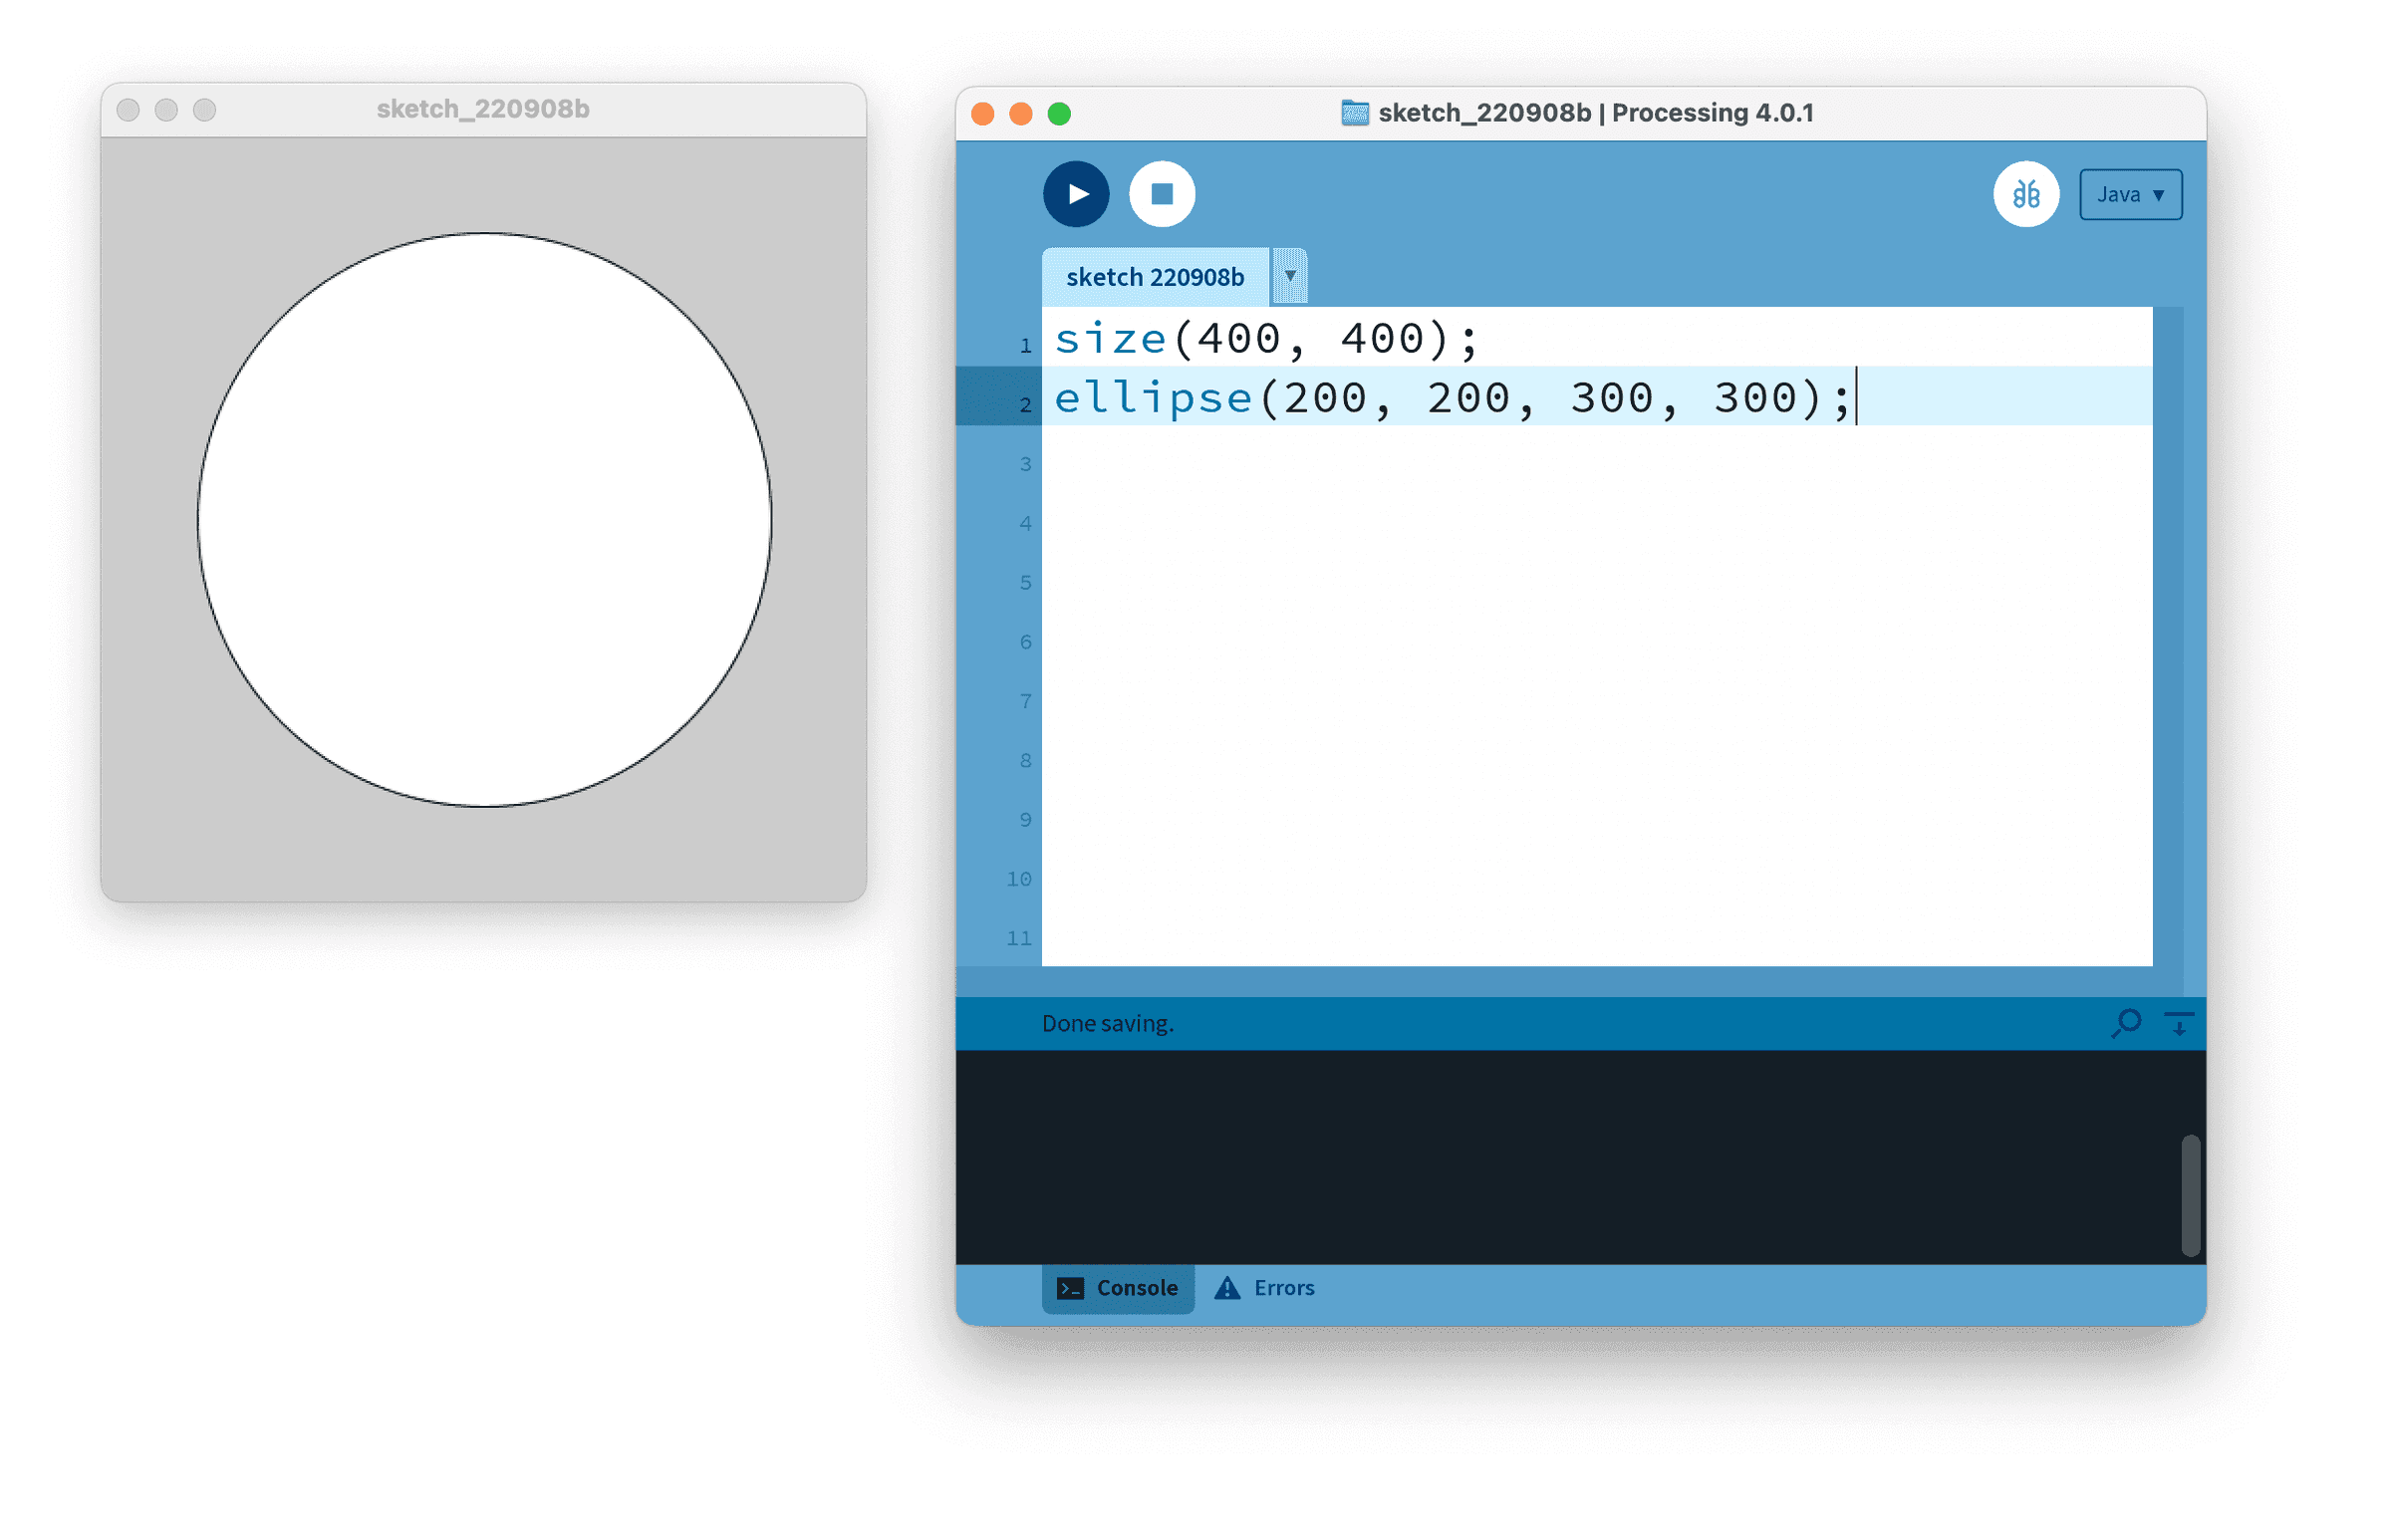
\includegraphics[width=1\textwidth]{images/processing_ide.png} 
    \caption[Processing IDE]{Processing IDE \parencite{reasProcessingIDE2015}}
    \label{fig:processing_ide_screenshot}
  \end{figure}

\subsection{The Legacy of Processing}
Processing is an open-source sketchbook and toolkit tailored for the electronic arts, new media art, and visual design communities, emphasizing the teaching of computer programming fundamentals within a visual context. Since its initial release on August 9, 2001 \parencite{processingfoundation20thAnniversaryProcessing2022}, Processing has had a lasting impact on computational design and creative coding.

This platform has not only persisted for over two decades but has also seen an expansion in its user base, indicating its continued relevance in a rapidly evolving field. Its role in shaping software literacy and education, especially for beginners, is well-documented, with its straightforward approach to coding and design principles that resonate with Maeda’s laws of simplicity \parencite{maedaJohnMaedaLaws2006}.

The platform’s design ethos of \enquote{Low Threshold, High Ceiling and Wide Walls} principles, has facilitated a nurturing environment for learning and creation \parencite{resnickDesignPrinciplesTools2005}. As indicated by user downloads that align with academic calendars \parencite{fryModernPrometheusHistory2018}, the steady increase in the adoption of Processing underscores its integration into educational structures. These metrics, alongside community surveys, suggest that Processing has transcended its educational utility, finding a place in artists’, designers’, and developers’ professional workflows \parencite{processingfoundation2016CommunitySurvey2016}.

Processing’s contribution to the field is further underlined by its influence on other significant projects, such as Wiring or Arduino, the microcontroller equivalent of Processing, which has roots in the same ethos and community \parencite{barraganUntoldHistoryArduino2016}. Its interface adaptability is evident through its evolution into variants like p5.js, Processing for Android, and Processing for Python, suggesting a responsive growth to the needs of its community, as visible on the Processing website. \parencite{processingfoundationProcessingWebsite}

Given its historical context and the progressive adaptation to user needs, Processing is a distinguished example of enduring software in the computational design and creative coding community. This longevity and adaptability call for a closer examination of its design philosophy and community dynamics. As we witness the retirement of once-pivotal tools like Flash or Director, Processing’s sustained relevance raises questions about the factors contributing to its success. \parencite{hortonDeathTechnicalSkill2020} \parencite{jobsThoughtsFlash2010} \parencite{adobecreativecloudteamFutureAdobeContribute2017}.

However, despite its success and influence, a concerning aspect is the project’s sustainability, considering the reliance on a small number of volunteer developers for most of the codebase \parencite{fryModernPrometheusHistory2018}. This situation poses significant questions about the long-term viability of open-source projects that are driven by community rather than commercial support.

\subsection{Research Questions}
The preceding section contextualized Processing as an influential tool that has withstood the test of time, promulgating computational design and creative coding. The software project, however, does not exist in isolation, as per Ben Fry’s insightful statement :

\begin{quote}
  \enquote{The processing project is a community, a piece of software that you run, and a language. And that order is important.} – Ben Fry \parencite[19:22]{artsatmit2017CASTSymposium2017}
\end{quote}\label{fry_quote}

This thesis seeks to unearth the necessary dynamics that underpin the formation and perpetuation of such a rich ecosystem around open-source software such as Processing. As such, the investigation pivots around a central research question:

\begin{quote}
  \enquote{What were the foundational dynamics that not only instigated but also sustained the collaborative spirit of the Processing community? Moreover, how did these dynamics, entwined with the intrinsic motivations of open-source contributors, influence the evolution of Processing’s software development over the years?}
\end{quote}

This question aims to dissect the symbiotic relationship between community involvement and software innovation, probing into how the motivations of volunteer contributors shaped the trajectory of Processing’s growth. The thesis will examine:

\begin{itemize}
\item The initial factors that attracted contributors to Processing and the elements that fostered their long-term engagement, as indicated by Fry’s prioritization of the community.
\item The various forms of contributions made to the project, from coding to forum participation, reflecting the intertwined nature of the software and language.
\item The transformation of these community dynamics from the nascent stages of Processing to its present-day stature.
\item The underpinning reasons for continued voluntary participation in the project’s development, despite the absence of direct financial incentives, aligning with Fry’s understanding of the community’s primacy.
\end{itemize}

Processing stands out from typical open-source software communities often studied because it is a Creativity Support Tool for the visual arts \parencite{shneidermanCreativitySupportTools2002}. Its main aim is to enhance the creative abilities of its users. This purpose departs from the practical goals usually central to well-studied, large-scale open-source communities, like those involved in the Linux Kernel development, which are frequently examined through models like the Cathedral and the Bazaar \parencite{raymondCathedralBazaarMusings2002}.
The findings from this investigation will broaden our comprehension of how sustainable, collaborative, open-source software initiatives can be developed specifically for creative applications.

\subsection{Information Sources}

% Research Design
Given the potential for memory bias due to the passage of time since the project’s inception, this thesis employs a mixed-methods approach. While human memory can be fallible, introducing biases and even constructing false memories, quantitative analysis serves as a foundational component to mitigate these challenges. It allows for identifying key contributors based on metrics such as software version control commit frequency, forum participation, and library contributions. These quantitative findings inform the selection of interview subjects, acting as a preliminary filter to locate contributors for qualitative interviews.
By purposefully integrating quantitative methodologies with qualitative ethnographic approaches, this research aspires to offer a nuanced understanding of both the structural and phenomenological aspects of the Processing community.

% Data Sources
The research draws upon multiple data sources to comprehensively understand the Processing community and its development practices—from forum discussions at various project phases to software version control logs and issue tracker reporting. The parsing status in Table~\ref{tab:data-sources} indicates the extent to which each data source has been prepared for analysis. 
%\begin{table}[h]
    \raggedright
    \caption{Data sources}
    \label{table:data-sources}
    \begin{tabular}{l l l c}
        \toprule
        Name & Type & Status \\
        \midrule
        Processing alpha forum & Forum & Parsed \\
        Processing beta forum & Forum & Parsed  \\
        Processing 1.0 forum & Forum & Downloaded \\
        Processing 2.0 and 3.0 forum & Forum  & Not downloaded \\
        Current processing forum & Forum & Not downloaded\\
        Github project & Commit history & Parsed \\
        Processing Release Data & Release notes & Parsed \\
        Github Release Data & Release notes \& download statistics & Parsed \\
        Processing libraries\textsuperscript{*} & Software release information & Parsed \\

        \bottomrule
        \multicolumn{3}{l}{\footnotesize \textsuperscript{*}Note: The data set was reconstructed from the processing website archive and is not complete.}
    \end{tabular}
  \end{table}      

\begin{table}
    \begin{adjustbox}{center}
    \begin{tabular}{l l l}
        \toprule
        Name & Type & Status \\
        \midrule
        Processing alpha forum & Forum & Parsed \\
        Processing beta forum & Forum & Parsed  \\
        Processing 1.0 forum & Forum & Parsed \\
        Processing 2.0 and 3.0 forum & Forum  & Downloaded \\
        Current processing forum & Forum & Downloaded \\
        Github project & Commit history & Parsed \\
        Processing Release Data & Release notes & Parsed \\
        Github Release Data & Release notes \& download statistics & Parsed \\
        Processing libraries\textsuperscript{*} & Software release information & Parsed \\
        Bugzilla & Software issue tracker & Not downloaded \\
        Github Issues & Software issue tracker & Not downloaded \\
        \bottomrule
        %\multicolumn{3}{l}{\footnotesize \textsuperscript{*}Note: }
    \end{tabular}
    \end{adjustbox}
    \caption[Data Sources]{Overview of Data Sources Used for Analyzing the Processing Community\\(\textsuperscript{*} The dataset is derived from an archival processing website and is incomplete.)}
    \label{tab:data-sources}
  \end{table}

% Software related discussions
% todo - add back maybe ????
% Initially, software-related discussions were confined to these forums. However, as the project matured, the complexity of issues warranted more specialized platforms for effective tracking and resolution. Consequently, the community transitioned from forums to Bugzilla \parencite{ProcessingBugzillaArchive2010} and eventually to GitHub Issues\parencite{processingfoundationProcessingSourceCode2020}
% \parencite{ProcessingProcessing4Processing}. 


% \begin{figure}[H]
%     \begin{minipage}{\textwidth}
%       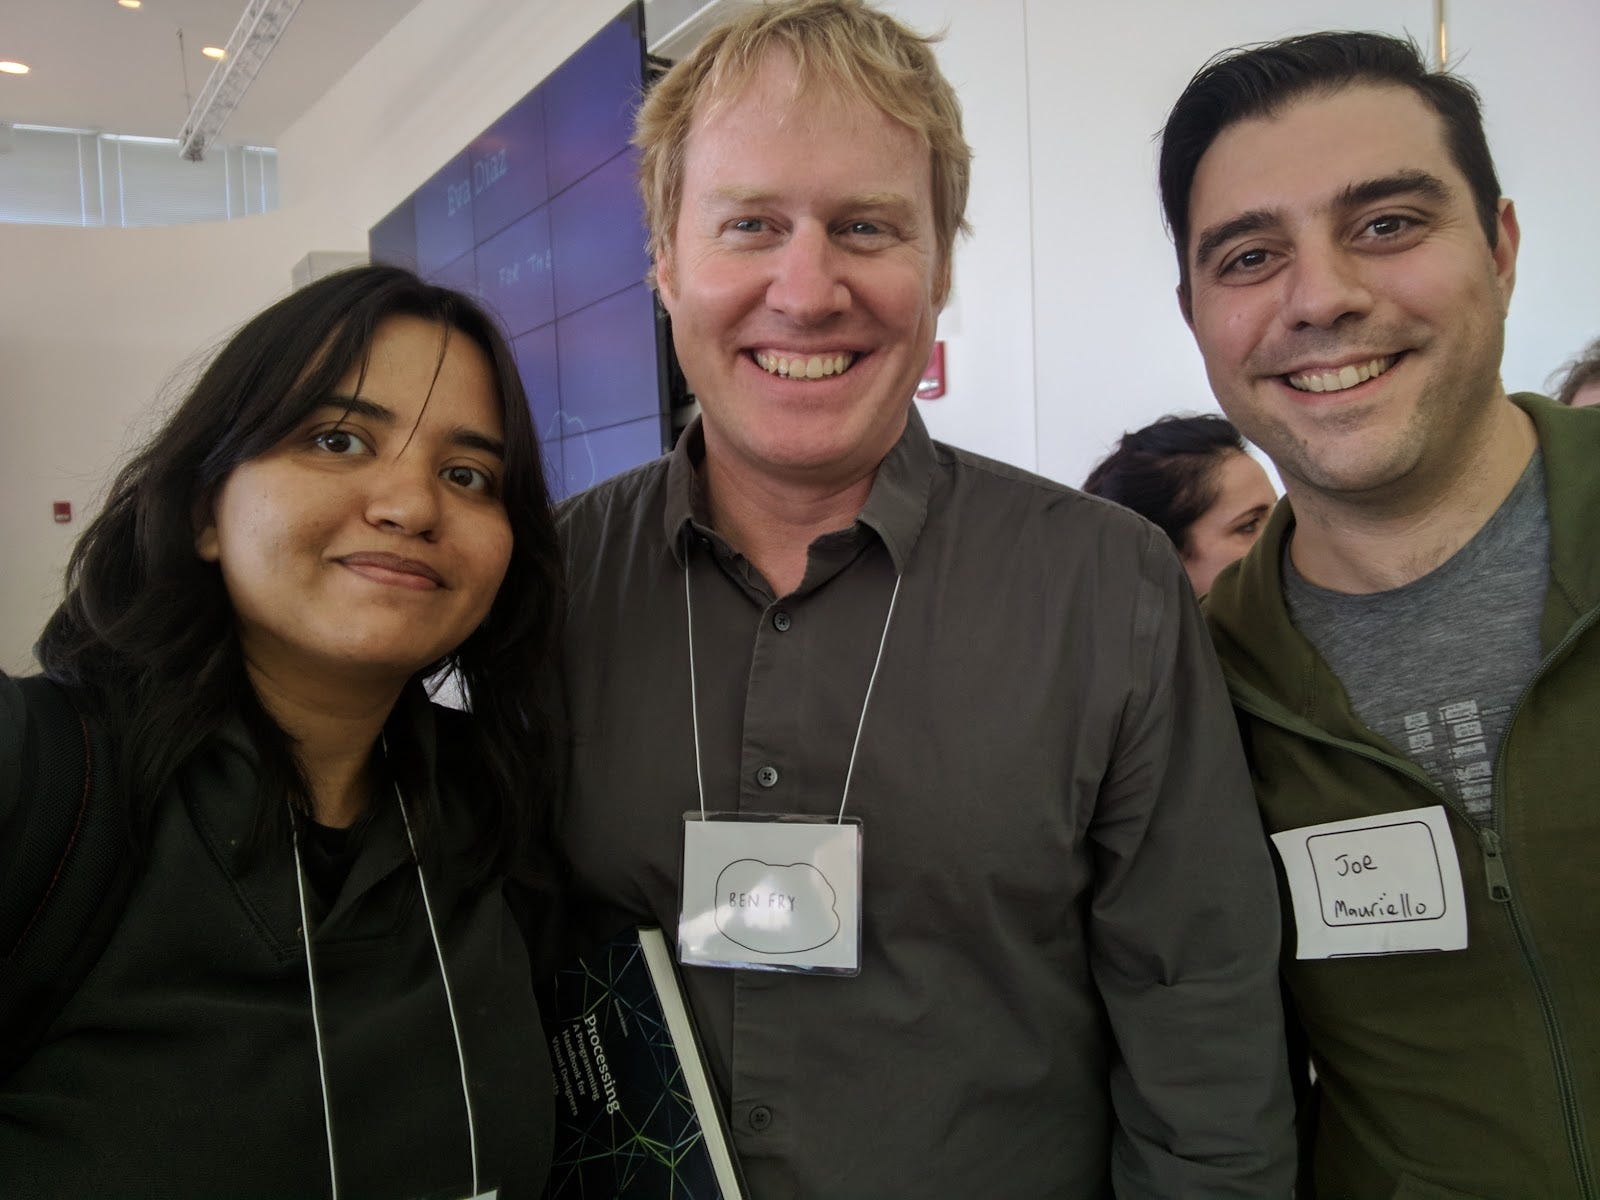
\includegraphics[width=\linewidth]{images/pcd2018.jpg}
%       \caption[Ben Fry at PCD 2018]{Ben Fry with conference atendees at Processing Community Day 2018. \fullcitefigure{guptaBenFryConference2018}.}
%       \label{fig:benFry}
%     \end{minipage}
%   \end{figure}
  
Interviewees were selected based on a strategic analysis of the collected data, especially in data-rich areas. Given the considerable quantity of data for the scope of the research project, particular attention was given to the project’s origin, precisely the period of activity before and during the activity of the initial alpha forum. The selection yielded three main categories of interview subjects:
  
\begin{itemize}
    \item Code contributors to the core project during the activity period of the initial alpha forum, from August 2, 2002, to April 19, 2005.
    \item Active forum members during the same time frame.
    \item Active library authors with frequent software release activity spanning from October 26, 2011, to June 8, 2014, based on available data
\end{itemize}


  \begin{table}[ht]
    \begin{adjustbox}{center}
    \begin{tabular}{lll}
    \hline
    Interviewee & Main Contribution & Date \\ \hline
    Jacob Schwartz (benelek) & Alpha forum participant & 2023-10-25 \\
    Ariel Malka (arielm) & Alpha forum participant & 2023-10-25 \\
    Ricard Marxer (Geomerative) & Library contributor & 2023-10-26 \\
    Simon Greenwold & Early contributor, ACG member & 2023-10-27 \\
    Martin Gomez (MartinG) & Alpha forum participant & 2023-10-30 \\
    Andreas Schlegel & ControlP5, oscP5 library contributor & 2023-10-31 \\
    Karsten Schmidt & Code and library contributor & 2023-11-07 \\
    Ben Fry & Processing co-founder & 2023-11-14 \\
    \hline
    \end{tabular}
    \label{tab:interviews}
\end{adjustbox}

    \caption[Contributor interviews]{Contributor interviews}
    \label{tab:interviews}

\end{table}
    
The primary qualitative method utilized was semi-structured interviews. The questions focused on how the individuals got involved, interacted with the community, perceived community dynamics, and their motivations to contribute. This choice was driven by the need for a flexible yet organized approach to gather in-depth insights from participants.

The qualitative insights gathered through interviews are essential in this research, allowing for a deeper understanding of the personal motivations and experiences of the contributors. Table \ref{tab:interviews} presents the names and roles of specific interview subjects to provide a comprehensive view of the primary sources that inform the analysis. Each interviewee was selected based on their unique contributions and roles in the Processing community, offering diverse perspectives that underpin the analysis of the following chapters. These dialogues not only reflect the quantitative data but also provide nuances that numbers alone cannot capture, thus enriching the narrative of this thesis.

However, the richness of these qualitative accounts brings into focus the scope and boundaries of the study. One of the most significant limitations is that it only covers a specific time frame and certain aspects of the Processing ecosystem. For instance, the research does not comprehensively cover all the noteworthy contributors to the Processing ecosystem. The individuals engaged primarily in writing documentation, examples, and books, those participating in or organizing local Processing Community Days or other community events, Google Summer of Code participants and mentors, and recipients of fellowship programs are all meaningful contributors to the ecosystem that fall outside the scope of this writing. Moreover, the research did not go into detail regarding the role of the Processing Foundation, a non-profit organization established to oversee the development and distribution of the processing software, in organizing the community and ensuring the sustainability of the Processing project. Therefore, it is critical to note that while the study has presented significant findings, it is not a comprehensive analysis.

\subsection{Structure}
This thesis adopts a structured approach to exploring the Processing project, guided by Ben Fry’s insightful quote as cited on page \pageref{fry_quote}. However, for this analysis, the examination will proceed in the reverse order of Fry’s listing—beginning with the language, moving to the software, and concluding with the community. This intentional inversion allows for a foundational understanding of the technical aspects before delving into the broader social and communal implications.

The first section focuses on the Processing language. It will delve into the syntax, structure, and unique aspects that make Processing an accessible yet powerful tool for creative coding. The evolution of the language from previous projects, such as Design by Numbers, will be examined and contextualized in the ecosystem of the tools of the time. 

Following the exploration of the language, the thesis will address the software development aspect of Processing. This section aims to unpack how the software was built and maintaned by the community.

The final section is dedicated to the community surrounding Processing. Here, the focus is on the growth, culture, and impact of the community around Processing. This section will investigate how community interactions, contributions, and collaborations have played a crucial role in shaping the project and expanding its reach and influence in computational design and creative coding.

By examining these components in this particular order, the thesis intends to build a layered understanding of Processing, from its technical core to its expansive community impact. This approach aims to provide a holistic view of the Processing project, showcasing how its technical aspects feed into and are influenced by its vibrant and dynamic community.